\documentclass[1p]{elsarticle_modified}
%\bibliographystyle{elsarticle-num}

%\usepackage[colorlinks]{hyperref}
%\usepackage{abbrmath_seonhwa} %\Abb, \Ascr, \Acal ,\Abf, \Afrak
\usepackage{amsfonts}
\usepackage{amssymb}
\usepackage{amsmath}
\usepackage{amsthm}
\usepackage{scalefnt}
\usepackage{amsbsy}
\usepackage{kotex}
\usepackage{caption}
\usepackage{subfig}
\usepackage{color}
\usepackage{graphicx}
\usepackage{xcolor} %% white, black, red, green, blue, cyan, magenta, yellow
\usepackage{float}
\usepackage{setspace}
\usepackage{hyperref}

\usepackage{tikz}
\usetikzlibrary{arrows}

\usepackage{multirow}
\usepackage{array} % fixed length table
\usepackage{hhline}

%%%%%%%%%%%%%%%%%%%%%
\makeatletter
\renewcommand*\env@matrix[1][\arraystretch]{%
	\edef\arraystretch{#1}%
	\hskip -\arraycolsep
	\let\@ifnextchar\new@ifnextchar
	\array{*\c@MaxMatrixCols c}}
\makeatother %https://tex.stackexchange.com/questions/14071/how-can-i-increase-the-line-spacing-in-a-matrix
%%%%%%%%%%%%%%%

\usepackage[normalem]{ulem}

\newcommand{\msout}[1]{\ifmmode\text{\sout{\ensuremath{#1}}}\else\sout{#1}\fi}
%SOURCE: \msout is \stkout macro in https://tex.stackexchange.com/questions/20609/strikeout-in-math-mode

\newcommand{\cancel}[1]{
	\ifmmode
	{\color{red}\msout{#1}}
	\else
	{\color{red}\sout{#1}}
	\fi
}

\newcommand{\add}[1]{
	{\color{blue}\uwave{#1}}
}

\newcommand{\replace}[2]{
	\ifmmode
	{\color{red}\msout{#1}}{\color{blue}\uwave{#2}}
	\else
	{\color{red}\sout{#1}}{\color{blue}\uwave{#2}}
	\fi
}

\newcommand{\Sol}{\mathcal{S}} %segment
\newcommand{\D}{D} %diagram
\newcommand{\A}{\mathcal{A}} %arc


%%%%%%%%%%%%%%%%%%%%%%%%%%%%%5 test

\def\sl{\operatorname{\textup{SL}}(2,\Cbb)}
\def\psl{\operatorname{\textup{PSL}}(2,\Cbb)}
\def\quan{\mkern 1mu \triangleright \mkern 1mu}

\theoremstyle{definition}
\newtheorem{thm}{Theorem}[section]
\newtheorem{prop}[thm]{Proposition}
\newtheorem{lem}[thm]{Lemma}
\newtheorem{ques}[thm]{Question}
\newtheorem{cor}[thm]{Corollary}
\newtheorem{defn}[thm]{Definition}
\newtheorem{exam}[thm]{Example}
\newtheorem{rmk}[thm]{Remark}
\newtheorem{alg}[thm]{Algorithm}

\newcommand{\I}{\sqrt{-1}}
\begin{document}

%\begin{frontmatter}
%
%\title{Boundary parabolic representations of knots up to 8 crossings}
%
%%% Group authors per affiliation:
%\author{Yunhi Cho} 
%\address{Department of Mathematics, University of Seoul, Seoul, Korea}
%\ead{yhcho@uos.ac.kr}
%
%
%\author{Seonhwa Kim} %\fnref{s_kim}}
%\address{Center for Geometry and Physics, Institute for Basic Science, Pohang, 37673, Korea}
%\ead{ryeona17@ibs.re.kr}
%
%\author{Hyuk Kim}
%\address{Department of Mathematical Sciences, Seoul National University, Seoul 08826, Korea}
%\ead{hyukkim@snu.ac.kr}
%
%\author{Seokbeom Yoon}
%\address{Department of Mathematical Sciences, Seoul National University, Seoul, 08826,  Korea}
%\ead{sbyoon15@snu.ac.kr}
%
%\begin{abstract}
%We find all boundary parabolic representation of knots up to 8 crossings.
%
%\end{abstract}
%\begin{keyword}
%    \MSC[2010] 57M25 
%\end{keyword}
%
%\end{frontmatter}

%\linenumbers
%\tableofcontents
%
\newcommand\colored[1]{\textcolor{white}{\rule[-0.35ex]{0.8em}{1.4ex}}\kern-0.8em\color{red} #1}%
%\newcommand\colored[1]{\textcolor{white}{ #1}\kern-2.17ex	\textcolor{white}{ #1}\kern-1.81ex	\textcolor{white}{ #1}\kern-2.15ex\color{red}#1	}

{\Large $\underline{10_{97}~(K10a_{12})}$}

\setlength{\tabcolsep}{10pt}
\renewcommand{\arraystretch}{1.6}
\vspace{1cm}\begin{tabular}{m{100pt}>{\centering\arraybackslash}m{274pt}}
\multirow{5}{120pt}{
	\centering
	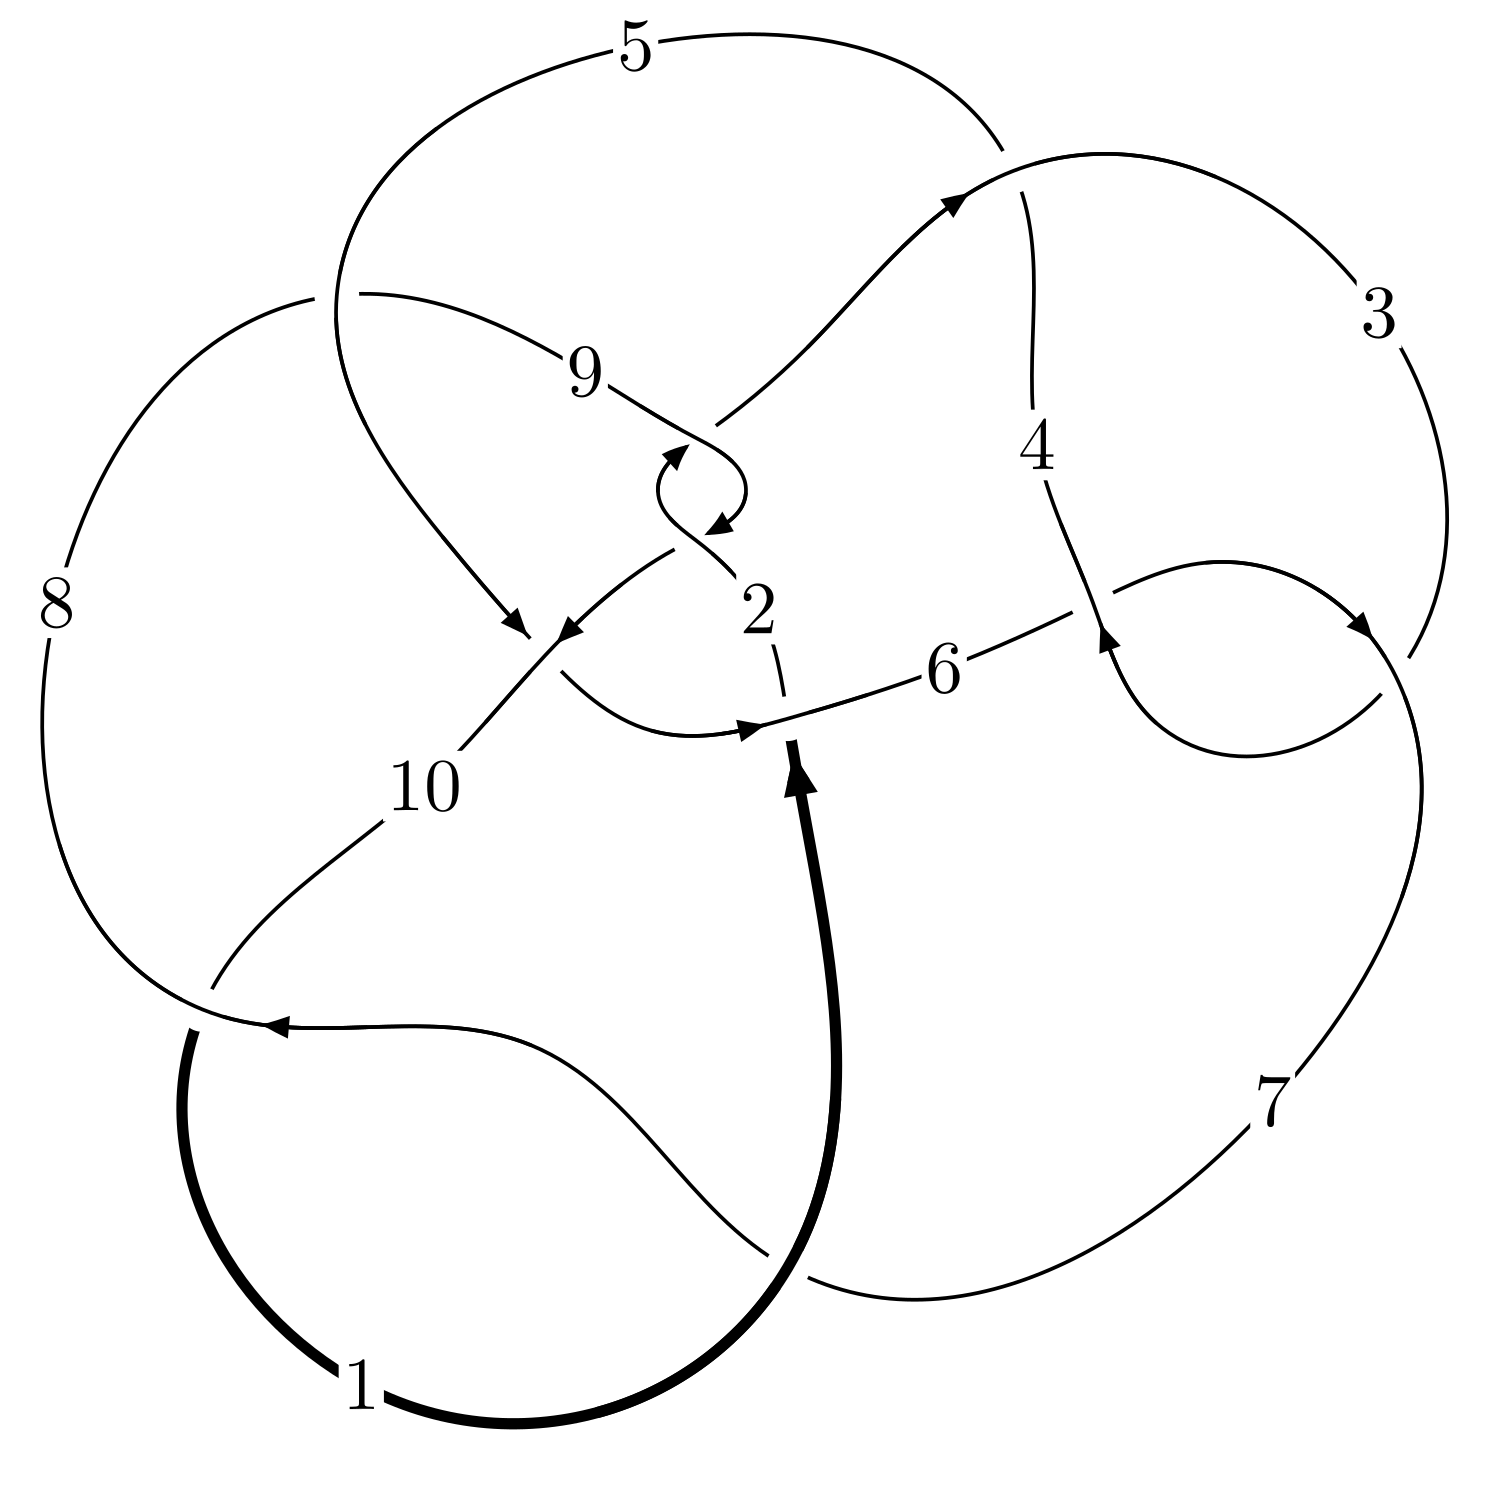
\includegraphics[width=112pt]{../../../GIT/diagram.site/Diagrams/png/181_10_97.png}\\
\ \ \ A knot diagram\footnotemark}&
\allowdisplaybreaks
\textbf{Linearized knot diagam} \\
\cline{2-2}
 &
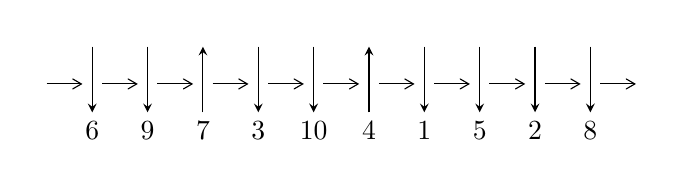
\begin{tikzpicture}[x=20pt, y=17pt]
	% nodes
	\node (C0) at (0, 0) {};
	\node (C1) at (1, 0) {};
	\node (C1U) at (1, +1) {};
	\node (C1D) at (1, -1) {6};

	\node (C2) at (2, 0) {};
	\node (C2U) at (2, +1) {};
	\node (C2D) at (2, -1) {9};

	\node (C3) at (3, 0) {};
	\node (C3U) at (3, +1) {};
	\node (C3D) at (3, -1) {7};

	\node (C4) at (4, 0) {};
	\node (C4U) at (4, +1) {};
	\node (C4D) at (4, -1) {3};

	\node (C5) at (5, 0) {};
	\node (C5U) at (5, +1) {};
	\node (C5D) at (5, -1) {10};

	\node (C6) at (6, 0) {};
	\node (C6U) at (6, +1) {};
	\node (C6D) at (6, -1) {4};

	\node (C7) at (7, 0) {};
	\node (C7U) at (7, +1) {};
	\node (C7D) at (7, -1) {1};

	\node (C8) at (8, 0) {};
	\node (C8U) at (8, +1) {};
	\node (C8D) at (8, -1) {5};

	\node (C9) at (9, 0) {};
	\node (C9U) at (9, +1) {};
	\node (C9D) at (9, -1) {2};

	\node (C10) at (10, 0) {};
	\node (C10U) at (10, +1) {};
	\node (C10D) at (10, -1) {8};
	\node (C11) at (11, 0) {};

	% arrows
	\draw[->,>={angle 60}]
	(C0) edge (C1) (C1) edge (C2) (C2) edge (C3) (C3) edge (C4) (C4) edge (C5) (C5) edge (C6) (C6) edge (C7) (C7) edge (C8) (C8) edge (C9) (C9) edge (C10) (C10) edge (C11) ;	\draw[->,>=stealth]
	(C1U) edge (C1D) (C2U) edge (C2D) (C3D) edge (C3U) (C4U) edge (C4D) (C5U) edge (C5D) (C6D) edge (C6U) (C7U) edge (C7D) (C8U) edge (C8D) (C9U) edge (C9D) (C10U) edge (C10D) ;
	\end{tikzpicture} \\
\hhline{~~} \\& 
\textbf{Solving Sequence} \\ \cline{2-2} 
 &
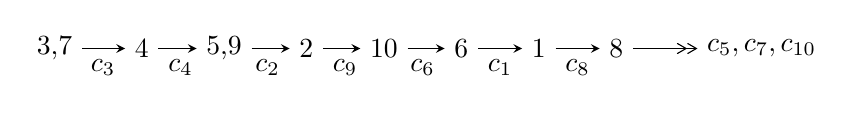
\begin{tikzpicture}[x=28pt, y=7pt]
	% node
	\node (A0) at (-1/8, 0) {3,7};
	\node (A1) at (1, 0) {4};
	\node (A2) at (33/16, 0) {5,9};
	\node (A3) at (25/8, 0) {2};
	\node (A4) at (33/8, 0) {10};
	\node (A5) at (41/8, 0) {6};
	\node (A6) at (49/8, 0) {1};
	\node (A7) at (57/8, 0) {8};
	\node (C1) at (1/2, -1) {$c_{3}$};
	\node (C2) at (3/2, -1) {$c_{4}$};
	\node (C3) at (21/8, -1) {$c_{2}$};
	\node (C4) at (29/8, -1) {$c_{9}$};
	\node (C5) at (37/8, -1) {$c_{6}$};
	\node (C6) at (45/8, -1) {$c_{1}$};
	\node (C7) at (53/8, -1) {$c_{8}$};
	\node (A8) at (9, 0) {$c_{5},c_{7},c_{10}$};

	% edge
	\draw[->,>=stealth]	
	(A0) edge (A1) (A1) edge (A2) (A2) edge (A3) (A3) edge (A4) (A4) edge (A5) (A5) edge (A6) (A6) edge (A7) ;
	\draw[->>,>={angle 60}]	
	(A7) edge (A8);
\end{tikzpicture} \\ 

\end{tabular} \\

\footnotetext{
The image of knot diagram is generated by the software ``\textbf{Draw programme}" developed by Andrew Bartholomew(\url{http://www.layer8.co.uk/maths/draw/index.htm\#Running-draw}), where we modified some parts for our purpose(\url{https://github.com/CATsTAILs/LinksPainter}).
}\phantom \\ \newline 
\centering \textbf{Ideals for irreducible components\footnotemark of $X_{\text{par}}$} 
 
\begin{align*}
I^u_{1}&=\langle 
2736614 u^{16}+18940720 u^{15}+\cdots+188712037 b-172998039,\\
\phantom{I^u_{1}}&\phantom{= \langle  }178471267 u^{16}+26934984 u^{15}+\cdots+754848148 a+1554469489,\\
\phantom{I^u_{1}}&\phantom{= \langle  }u^{17}+3 u^{15}+7 u^{13}+u^{12}+10 u^{11}+2 u^{10}+11 u^9+4 u^8+22 u^7-12 u^6+38 u^5-21 u^4+36 u^3-18 u^2+17 u-4\rangle \\
I^u_{2}&=\langle 
u^{13} a- u^{13}+\cdots+b-3,\;2 u^{13} a- u^{13}+\cdots+2 a-5,\\
\phantom{I^u_{2}}&\phantom{= \langle  }u^{14}- u^{13}+3 u^{12}-2 u^{11}+6 u^{10}-3 u^9+7 u^8-2 u^7+6 u^6+4 u^4+2 u^2+u+1\rangle \\
I^u_{3}&=\langle 
b+1,\;2 a-2 u-1,\;u^2+u+1\rangle \\
\\
\end{align*}
\raggedright * 3 irreducible components of $\dim_{\mathbb{C}}=0$, with total 47 representations.\\
\footnotetext{All coefficients of polynomials are rational numbers. But the coefficients are sometimes approximated in decimal forms when there is not enough margin.}
\newpage
\renewcommand{\arraystretch}{1}
\centering \section*{I. $I^u_{1}= \langle 2.74\times10^{6} u^{16}+1.89\times10^{7} u^{15}+\cdots+1.89\times10^{8} b-1.73\times10^{8},\;1.78\times10^{8} u^{16}+2.69\times10^{7} u^{15}+\cdots+7.55\times10^{8} a+1.55\times10^{9},\;u^{17}+3 u^{15}+\cdots+17 u-4 \rangle$}
\flushleft \textbf{(i) Arc colorings}\\
\begin{tabular}{m{7pt} m{180pt} m{7pt} m{180pt} }
\flushright $a_{3}=$&$\begin{pmatrix}1\\0\end{pmatrix}$ \\
\flushright $a_{7}=$&$\begin{pmatrix}0\\u\end{pmatrix}$ \\
\flushright $a_{4}=$&$\begin{pmatrix}1\\- u^2\end{pmatrix}$ \\
\flushright $a_{5}=$&$\begin{pmatrix}u^2+1\\- u^2\end{pmatrix}$ \\
\flushright $a_{9}=$&$\begin{pmatrix}-0.236433 u^{16}-0.0356827 u^{15}+\cdots+3.37770 u-2.05931\\-0.0145015 u^{16}-0.100368 u^{15}+\cdots-1.37842 u+0.916730\end{pmatrix}$ \\
\flushright $a_{2}=$&$\begin{pmatrix}0.252945 u^{16}+0.0144309 u^{15}+\cdots-3.32958 u+2.37418\\0.0316855 u^{16}+0.201926 u^{15}+\cdots+2.11952 u-0.917967\end{pmatrix}$ \\
\flushright $a_{10}=$&$\begin{pmatrix}-0.475929 u^{16}+0.0117484 u^{15}+\cdots+7.44839 u-3.87934\\-0.0117484 u^{16}-0.307312 u^{15}+\cdots-4.21145 u+1.90371\end{pmatrix}$ \\
\flushright $a_{6}=$&$\begin{pmatrix}- u\\u^3+u\end{pmatrix}$ \\
\flushright $a_{1}=$&$\begin{pmatrix}0.229183 u^{16}-0.0145015 u^{15}+\cdots-3.56691 u+2.51768\\-0.0356827 u^{16}+0.0837041 u^{15}+\cdots+1.96005 u-0.945733\end{pmatrix}$ \\
\flushright $a_{8}=$&$\begin{pmatrix}-0.229492 u^{16}+0.0316855 u^{15}+\cdots+3.85585 u-1.78184\\0.0144309 u^{16}-0.191499 u^{15}+\cdots-1.92588 u+1.01178\end{pmatrix}$\\&\end{tabular}
\flushleft \textbf{(ii) Obstruction class $= -1$}\\~\\
\flushleft \textbf{(iii) Cusp Shapes $= \frac{153304973}{188712037} u^{16}-\frac{89774747}{754848148} u^{15}+\cdots-\frac{9028153643}{754848148} u-\frac{1460399043}{188712037}$}\\~\\
\newpage\renewcommand{\arraystretch}{1}
\flushleft \textbf{(iv) u-Polynomials at the component}\newline \\
\begin{tabular}{m{50pt}|m{274pt}}
Crossings & \hspace{64pt}u-Polynomials at each crossing \\
\hline $$\begin{aligned}c_{1},c_{8}\end{aligned}$$&$\begin{aligned}
&4(4 u^{17}+2 u^{16}+\cdots+u^2+1)
\end{aligned}$\\
\hline $$\begin{aligned}c_{2},c_{7},c_{9}\\c_{10}\end{aligned}$$&$\begin{aligned}
&u^{17}+2 u^{16}+\cdots-2 u+1
\end{aligned}$\\
\hline $$\begin{aligned}c_{3},c_{6}\end{aligned}$$&$\begin{aligned}
&u^{17}+3 u^{15}+\cdots+17 u+4
\end{aligned}$\\
\hline $$\begin{aligned}c_{4}\end{aligned}$$&$\begin{aligned}
&u^{17}+6 u^{16}+\cdots+145 u-16
\end{aligned}$\\
\hline $$\begin{aligned}c_{5}\end{aligned}$$&$\begin{aligned}
&u^{17}-3 u^{16}+\cdots-24 u+32
\end{aligned}$\\
\hline
\end{tabular}\\~\\
\newpage\renewcommand{\arraystretch}{1}
\flushleft \textbf{(v) Riley Polynomials at the component}\newline \\
\begin{tabular}{m{50pt}|m{274pt}}
Crossings & \hspace{64pt}Riley Polynomials at each crossing \\
\hline $$\begin{aligned}c_{1},c_{8}\end{aligned}$$&$\begin{aligned}
&16(16 y^{17}+132 y^{16}+\cdots-2 y-1)
\end{aligned}$\\
\hline $$\begin{aligned}c_{2},c_{7},c_{9}\\c_{10}\end{aligned}$$&$\begin{aligned}
&y^{17}+10 y^{16}+\cdots+8 y-1
\end{aligned}$\\
\hline $$\begin{aligned}c_{3},c_{6}\end{aligned}$$&$\begin{aligned}
&y^{17}+6 y^{16}+\cdots+145 y-16
\end{aligned}$\\
\hline $$\begin{aligned}c_{4}\end{aligned}$$&$\begin{aligned}
&y^{17}+10 y^{16}+\cdots+44449 y-256
\end{aligned}$\\
\hline $$\begin{aligned}c_{5}\end{aligned}$$&$\begin{aligned}
&y^{17}+5 y^{16}+\cdots-6976 y-1024
\end{aligned}$\\
\hline
\end{tabular}\\~\\
\newpage\flushleft \textbf{(vi) Complex Volumes and Cusp Shapes}
$$\begin{array}{c|c|c}  
\text{Solutions to }I^u_{1}& \I (\text{vol} + \sqrt{-1}CS) & \text{Cusp shape}\\
 \hline 
\begin{aligned}
u &= -0.417221 + 0.885126 I \\
a &= -0.476552 + 0.009774 I \\
b &= -0.222604 + 0.163997 I\end{aligned}
 & -0.34103 - 1.75255 I & -2.16634 + 2.85736 I \\ \hline\begin{aligned}
u &= -0.417221 - 0.885126 I \\
a &= -0.476552 - 0.009774 I \\
b &= -0.222604 - 0.163997 I\end{aligned}
 & -0.34103 + 1.75255 I & -2.16634 - 2.85736 I \\ \hline\begin{aligned}
u &= \phantom{-}0.597620 + 0.869356 I \\
a &= -0.334759 + 0.962950 I \\
b &= \phantom{-}1.335870 + 0.125893 I\end{aligned}
 & -1.15632 + 2.35456 I & \phantom{-}2.48228 - 6.50501 I \\ \hline\begin{aligned}
u &= \phantom{-}0.597620 - 0.869356 I \\
a &= -0.334759 - 0.962950 I \\
b &= \phantom{-}1.335870 - 0.125893 I\end{aligned}
 & -1.15632 - 2.35456 I & \phantom{-}2.48228 + 6.50501 I \\ \hline\begin{aligned}
u &= \phantom{-}0.236791 + 0.896556 I \\
a &= \phantom{-}0.903548 + 1.016340 I \\
b &= \phantom{-}0.840094 - 0.523489 I\end{aligned}
 & -2.94308 + 1.91475 I & -12.50863 - 1.23884 I \\ \hline\begin{aligned}
u &= \phantom{-}0.236791 - 0.896556 I \\
a &= \phantom{-}0.903548 - 1.016340 I \\
b &= \phantom{-}0.840094 + 0.523489 I\end{aligned}
 & -2.94308 - 1.91475 I & -12.50863 + 1.23884 I \\ \hline\begin{aligned}
u &= \phantom{-}0.979244 + 0.594888 I \\
a &= \phantom{-}0.26940 + 1.57950 I \\
b &= -0.44756 - 1.37873 I\end{aligned}
 & \phantom{-}9.32990 - 8.56729 I & \phantom{-}0.17143 + 4.34513 I \\ \hline\begin{aligned}
u &= \phantom{-}0.979244 - 0.594888 I \\
a &= \phantom{-}0.26940 - 1.57950 I \\
b &= -0.44756 + 1.37873 I\end{aligned}
 & \phantom{-}9.32990 + 8.56729 I & \phantom{-}0.17143 - 4.34513 I \\ \hline\begin{aligned}
u &= -1.198530 + 0.485201 I \\
a &= -0.11385 + 1.41682 I \\
b &= -0.047500 - 1.229640 I\end{aligned}
 & \phantom{-}7.90214 - 1.97950 I & \phantom{-}6.13742 + 2.92595 I \\ \hline\begin{aligned}
u &= -1.198530 - 0.485201 I \\
a &= -0.11385 - 1.41682 I \\
b &= -0.047500 + 1.229640 I\end{aligned}
 & \phantom{-}7.90214 + 1.97950 I & \phantom{-}6.13742 - 2.92595 I\\
 \hline 
 \end{array}$$\newpage$$\begin{array}{c|c|c}  
\text{Solutions to }I^u_{1}& \I (\text{vol} + \sqrt{-1}CS) & \text{Cusp shape}\\
 \hline 
\begin{aligned}
u &= \phantom{-}0.745598 + 1.114110 I \\
a &= -1.29641 - 1.54585 I \\
b &= -0.53774 + 1.38258 I\end{aligned}
 & \phantom{-}7.7059 + 14.8527 I & -2.01529 - 8.44038 I \\ \hline\begin{aligned}
u &= \phantom{-}0.745598 - 1.114110 I \\
a &= -1.29641 + 1.54585 I \\
b &= -0.53774 - 1.38258 I\end{aligned}
 & \phantom{-}7.7059 - 14.8527 I & -2.01529 + 8.44038 I \\ \hline\begin{aligned}
u &= -0.203786 + 1.345170 I \\
a &= -0.540937 + 0.304824 I \\
b &= -0.347263 - 1.122360 I\end{aligned}
 & \phantom{-}1.26847 - 6.54787 I & -3.86293 + 7.90993 I \\ \hline\begin{aligned}
u &= -0.203786 - 1.345170 I \\
a &= -0.540937 - 0.304824 I \\
b &= -0.347263 + 1.122360 I\end{aligned}
 & \phantom{-}1.26847 + 6.54787 I & -3.86293 - 7.90993 I \\ \hline\begin{aligned}
u &= -0.87723 + 1.18507 I \\
a &= \phantom{-}0.723215 - 1.188380 I \\
b &= \phantom{-}0.161092 + 1.190930 I\end{aligned}
 & \phantom{-}5.81019 - 5.32225 I & \phantom{-}2.45956 + 7.34338 I \\ \hline\begin{aligned}
u &= -0.87723 - 1.18507 I \\
a &= \phantom{-}0.723215 + 1.188380 I \\
b &= \phantom{-}0.161092 - 1.190930 I\end{aligned}
 & \phantom{-}5.81019 + 5.32225 I & \phantom{-}2.45956 - 7.34338 I \\ \hline\begin{aligned}
u &= \phantom{-}0.275016\phantom{ +0.000000I} \\
a &= -1.51732\phantom{ +0.000000I} \\
b &= \phantom{-}0.531228\phantom{ +0.000000I}\end{aligned}
 & -0.869406\phantom{ +0.000000I} & -11.1450\phantom{ +0.000000I}\\
 \hline 
 \end{array}$$\newpage\newpage\renewcommand{\arraystretch}{1}
\centering \section*{II. $I^u_{2}= \langle u^{13} a- u^{13}+\cdots+b-3,\;2 u^{13} a- u^{13}+\cdots+2 a-5,\;u^{14}- u^{13}+\cdots+u+1 \rangle$}
\flushleft \textbf{(i) Arc colorings}\\
\begin{tabular}{m{7pt} m{180pt} m{7pt} m{180pt} }
\flushright $a_{3}=$&$\begin{pmatrix}1\\0\end{pmatrix}$ \\
\flushright $a_{7}=$&$\begin{pmatrix}0\\u\end{pmatrix}$ \\
\flushright $a_{4}=$&$\begin{pmatrix}1\\- u^2\end{pmatrix}$ \\
\flushright $a_{5}=$&$\begin{pmatrix}u^2+1\\- u^2\end{pmatrix}$ \\
\flushright $a_{9}=$&$\begin{pmatrix}a\\- u^{13} a+u^{13}+\cdots-2 u+3\end{pmatrix}$ \\
\flushright $a_{2}=$&$\begin{pmatrix}u^{13} a+6 u^{13}+\cdots+3 a+6\\- u^{13} a- u^{13}+\cdots- a+1\end{pmatrix}$ \\
\flushright $a_{10}=$&$\begin{pmatrix}u^{13}+2 u^{11}+3 u^9+2 u^7- u\\- u^{13}+u^{12}-2 u^{11}+3 u^{10}-3 u^9+5 u^8-2 u^7+6 u^6+4 u^4+3 u^2+u+1\end{pmatrix}$ \\
\flushright $a_{6}=$&$\begin{pmatrix}- u\\u^3+u\end{pmatrix}$ \\
\flushright $a_{1}=$&$\begin{pmatrix}u^{12} a+3 u^{13}+\cdots+2 a+6\\2 u^{13}-2 u^{12}+\cdots- a u+2\end{pmatrix}$ \\
\flushright $a_{8}=$&$\begin{pmatrix}- u^{13} a- u^{13}+\cdots- a+1\\- u^{13} a+2 u^{13}+\cdots+a+4\end{pmatrix}$\\&\end{tabular}
\flushleft \textbf{(ii) Obstruction class $= -1$}\\~\\
\flushleft \textbf{(iii) Cusp Shapes $= -4 u^{12}+4 u^{11}-8 u^{10}+8 u^9-16 u^8+12 u^7-12 u^6+12 u^5-8 u^4+4 u^3-4 u^2+8 u-2$}\\~\\
\newpage\renewcommand{\arraystretch}{1}
\flushleft \textbf{(iv) u-Polynomials at the component}\newline \\
\begin{tabular}{m{50pt}|m{274pt}}
Crossings & \hspace{64pt}u-Polynomials at each crossing \\
\hline $$\begin{aligned}c_{1},c_{8}\end{aligned}$$&$\begin{aligned}
&u^{28}-3 u^{27}+\cdots-1254 u+653
\end{aligned}$\\
\hline $$\begin{aligned}c_{2},c_{7},c_{9}\\c_{10}\end{aligned}$$&$\begin{aligned}
&u^{28}-5 u^{27}+\cdots-2 u+1
\end{aligned}$\\
\hline $$\begin{aligned}c_{3},c_{5},c_{6}\end{aligned}$$&$\begin{aligned}
&(u^{14}+u^{13}+\cdots- u+1)^{2}
\end{aligned}$\\
\hline $$\begin{aligned}c_{4}\end{aligned}$$&$\begin{aligned}
&(u^{14}+5 u^{13}+\cdots+3 u+1)^{2}
\end{aligned}$\\
\hline
\end{tabular}\\~\\
\newpage\renewcommand{\arraystretch}{1}
\flushleft \textbf{(v) Riley Polynomials at the component}\newline \\
\begin{tabular}{m{50pt}|m{274pt}}
Crossings & \hspace{64pt}Riley Polynomials at each crossing \\
\hline $$\begin{aligned}c_{1},c_{8}\end{aligned}$$&$\begin{aligned}
&y^{28}+15 y^{27}+\cdots+3659320 y+426409
\end{aligned}$\\
\hline $$\begin{aligned}c_{2},c_{7},c_{9}\\c_{10}\end{aligned}$$&$\begin{aligned}
&y^{28}+19 y^{27}+\cdots-10 y^2+1
\end{aligned}$\\
\hline $$\begin{aligned}c_{3},c_{5},c_{6}\end{aligned}$$&$\begin{aligned}
&(y^{14}+5 y^{13}+\cdots+3 y+1)^{2}
\end{aligned}$\\
\hline $$\begin{aligned}c_{4}\end{aligned}$$&$\begin{aligned}
&(y^{14}+9 y^{13}+\cdots+15 y+1)^{2}
\end{aligned}$\\
\hline
\end{tabular}\\~\\
\newpage\flushleft \textbf{(vi) Complex Volumes and Cusp Shapes}
$$\begin{array}{c|c|c}  
\text{Solutions to }I^u_{2}& \I (\text{vol} + \sqrt{-1}CS) & \text{Cusp shape}\\
 \hline 
\begin{aligned}
u &= \phantom{-}0.772300 + 0.626535 I \\
a &= \phantom{-}0.406503 - 0.509972 I \\
b &= -1.027090 - 0.175615 I\end{aligned}
 & \phantom{-}4.48016 - 3.41271 I & -1.89400 + 2.62516 I \\ \hline\begin{aligned}
u &= \phantom{-}0.772300 + 0.626535 I \\
a &= -0.59492 - 1.65604 I \\
b &= \phantom{-}0.41210 + 1.42136 I\end{aligned}
 & \phantom{-}4.48016 - 3.41271 I & -1.89400 + 2.62516 I \\ \hline\begin{aligned}
u &= \phantom{-}0.772300 - 0.626535 I \\
a &= \phantom{-}0.406503 + 0.509972 I \\
b &= -1.027090 + 0.175615 I\end{aligned}
 & \phantom{-}4.48016 + 3.41271 I & -1.89400 - 2.62516 I \\ \hline\begin{aligned}
u &= \phantom{-}0.772300 - 0.626535 I \\
a &= -0.59492 + 1.65604 I \\
b &= \phantom{-}0.41210 - 1.42136 I\end{aligned}
 & \phantom{-}4.48016 + 3.41271 I & -1.89400 - 2.62516 I \\ \hline\begin{aligned}
u &= -0.050221 + 1.076790 I \\
a &= -0.752996 - 0.510112 I \\
b &= -0.637817 + 0.252286 I\end{aligned}
 & -1.35286 - 2.76747 I & -9.41762 + 3.21377 I \\ \hline\begin{aligned}
u &= -0.050221 + 1.076790 I \\
a &= \phantom{-}0.315982 + 0.198126 I \\
b &= \phantom{-}0.426047 + 1.000290 I\end{aligned}
 & -1.35286 - 2.76747 I & -9.41762 + 3.21377 I \\ \hline\begin{aligned}
u &= -0.050221 - 1.076790 I \\
a &= -0.752996 + 0.510112 I \\
b &= -0.637817 - 0.252286 I\end{aligned}
 & -1.35286 + 2.76747 I & -9.41762 - 3.21377 I \\ \hline\begin{aligned}
u &= -0.050221 - 1.076790 I \\
a &= \phantom{-}0.315982 - 0.198126 I \\
b &= \phantom{-}0.426047 - 1.000290 I\end{aligned}
 & -1.35286 + 2.76747 I & -9.41762 - 3.21377 I \\ \hline\begin{aligned}
u &= \phantom{-}0.727524 + 0.860849 I \\
a &= \phantom{-}0.715949 + 1.174200 I \\
b &= -0.51211 - 1.46812 I\end{aligned}
 & \phantom{-}7.93259 + 2.76747 I & \phantom{-}1.41762 - 3.21377 I \\ \hline\begin{aligned}
u &= \phantom{-}0.727524 + 0.860849 I \\
a &= -1.19732 - 1.74297 I \\
b &= -0.64484 + 1.35997 I\end{aligned}
 & \phantom{-}7.93259 + 2.76747 I & \phantom{-}1.41762 - 3.21377 I\\
 \hline 
 \end{array}$$\newpage$$\begin{array}{c|c|c}  
\text{Solutions to }I^u_{2}& \I (\text{vol} + \sqrt{-1}CS) & \text{Cusp shape}\\
 \hline 
\begin{aligned}
u &= \phantom{-}0.727524 - 0.860849 I \\
a &= \phantom{-}0.715949 - 1.174200 I \\
b &= -0.51211 + 1.46812 I\end{aligned}
 & \phantom{-}7.93259 - 2.76747 I & \phantom{-}1.41762 + 3.21377 I \\ \hline\begin{aligned}
u &= \phantom{-}0.727524 - 0.860849 I \\
a &= -1.19732 + 1.74297 I \\
b &= -0.64484 - 1.35997 I\end{aligned}
 & \phantom{-}7.93259 - 2.76747 I & \phantom{-}1.41762 + 3.21377 I \\ \hline\begin{aligned}
u &= -0.494052 + 0.663856 I \\
a &= \phantom{-}0.96368 - 1.66194 I \\
b &= \phantom{-}0.053811 - 0.680241 I\end{aligned}
 & \phantom{-}3.26705 - 1.37770 I & -4.88590 + 4.12207 I \\ \hline\begin{aligned}
u &= -0.494052 + 0.663856 I \\
a &= -0.95490 - 2.71701 I \\
b &= \phantom{-}0.006983 + 1.150230 I\end{aligned}
 & \phantom{-}3.26705 - 1.37770 I & -4.88590 + 4.12207 I \\ \hline\begin{aligned}
u &= -0.494052 - 0.663856 I \\
a &= \phantom{-}0.96368 + 1.66194 I \\
b &= \phantom{-}0.053811 + 0.680241 I\end{aligned}
 & \phantom{-}3.26705 + 1.37770 I & -4.88590 - 4.12207 I \\ \hline\begin{aligned}
u &= -0.494052 - 0.663856 I \\
a &= -0.95490 + 2.71701 I \\
b &= \phantom{-}0.006983 - 1.150230 I\end{aligned}
 & \phantom{-}3.26705 + 1.37770 I & -4.88590 - 4.12207 I \\ \hline\begin{aligned}
u &= -0.622207 + 1.001070 I \\
a &= \phantom{-}0.372140 + 0.404462 I \\
b &= \phantom{-}0.340282 + 0.137082 I\end{aligned}
 & \phantom{-}2.09958 - 3.41271 I & -6.10600 + 2.62516 I \\ \hline\begin{aligned}
u &= -0.622207 + 1.001070 I \\
a &= -1.58493 + 1.41489 I \\
b &= -0.136381 - 1.104830 I\end{aligned}
 & \phantom{-}2.09958 - 3.41271 I & -6.10600 + 2.62516 I \\ \hline\begin{aligned}
u &= -0.622207 - 1.001070 I \\
a &= \phantom{-}0.372140 - 0.404462 I \\
b &= \phantom{-}0.340282 - 0.137082 I\end{aligned}
 & \phantom{-}2.09958 + 3.41271 I & -6.10600 - 2.62516 I \\ \hline\begin{aligned}
u &= -0.622207 - 1.001070 I \\
a &= -1.58493 - 1.41489 I \\
b &= -0.136381 + 1.104830 I\end{aligned}
 & \phantom{-}2.09958 + 3.41271 I & -6.10600 - 2.62516 I\\
 \hline 
 \end{array}$$\newpage$$\begin{array}{c|c|c}  
\text{Solutions to }I^u_{2}& \I (\text{vol} + \sqrt{-1}CS) & \text{Cusp shape}\\
 \hline 
\begin{aligned}
u &= \phantom{-}0.683715 + 1.025590 I \\
a &= \phantom{-}0.010710 - 0.783806 I \\
b &= -1.148810 + 0.016311 I\end{aligned}
 & \phantom{-}3.28987 + 8.93586 I & -4.00000 - 7.26077 I \\ \hline\begin{aligned}
u &= \phantom{-}0.683715 + 1.025590 I \\
a &= \phantom{-}1.32082 + 1.63940 I \\
b &= \phantom{-}0.56444 - 1.41873 I\end{aligned}
 & \phantom{-}3.28987 + 8.93586 I & -4.00000 - 7.26077 I \\ \hline\begin{aligned}
u &= \phantom{-}0.683715 - 1.025590 I \\
a &= \phantom{-}0.010710 + 0.783806 I \\
b &= -1.148810 - 0.016311 I\end{aligned}
 & \phantom{-}3.28987 - 8.93586 I & -4.00000 + 7.26077 I \\ \hline\begin{aligned}
u &= \phantom{-}0.683715 - 1.025590 I \\
a &= \phantom{-}1.32082 - 1.63940 I \\
b &= \phantom{-}0.56444 + 1.41873 I\end{aligned}
 & \phantom{-}3.28987 - 8.93586 I & -4.00000 + 7.26077 I \\ \hline\begin{aligned}
u &= -0.517057 + 0.454483 I \\
a &= -0.163546 - 1.319840 I \\
b &= -0.212363 - 0.520130 I\end{aligned}
 & \phantom{-}3.31269 - 1.37770 I & -3.11410 + 4.12207 I \\ \hline\begin{aligned}
u &= -0.517057 + 0.454483 I \\
a &= -0.85718 - 1.74842 I \\
b &= \phantom{-}0.015745 + 1.176090 I\end{aligned}
 & \phantom{-}3.31269 - 1.37770 I & -3.11410 + 4.12207 I \\ \hline\begin{aligned}
u &= -0.517057 - 0.454483 I \\
a &= -0.163546 + 1.319840 I \\
b &= -0.212363 + 0.520130 I\end{aligned}
 & \phantom{-}3.31269 + 1.37770 I & -3.11410 - 4.12207 I \\ \hline\begin{aligned}
u &= -0.517057 - 0.454483 I \\
a &= -0.85718 + 1.74842 I \\
b &= \phantom{-}0.015745 - 1.176090 I\end{aligned}
 & \phantom{-}3.31269 + 1.37770 I & -3.11410 - 4.12207 I\\
 \hline 
 \end{array}$$\newpage\newpage\renewcommand{\arraystretch}{1}
\centering \section*{III. $I^u_{3}= \langle b+1,\;2 a-2 u-1,\;u^2+u+1 \rangle$}
\flushleft \textbf{(i) Arc colorings}\\
\begin{tabular}{m{7pt} m{180pt} m{7pt} m{180pt} }
\flushright $a_{3}=$&$\begin{pmatrix}1\\0\end{pmatrix}$ \\
\flushright $a_{7}=$&$\begin{pmatrix}0\\u\end{pmatrix}$ \\
\flushright $a_{4}=$&$\begin{pmatrix}1\\u+1\end{pmatrix}$ \\
\flushright $a_{5}=$&$\begin{pmatrix}- u\\u+1\end{pmatrix}$ \\
\flushright $a_{9}=$&$\begin{pmatrix}u+\frac{1}{2}\\-1\end{pmatrix}$ \\
\flushright $a_{2}=$&$\begin{pmatrix}u+\frac{3}{2}\\-1\end{pmatrix}$ \\
\flushright $a_{10}=$&$\begin{pmatrix}2 u+2\\-2\end{pmatrix}$ \\
\flushright $a_{6}=$&$\begin{pmatrix}- u\\u+1\end{pmatrix}$ \\
\flushright $a_{1}=$&$\begin{pmatrix}u+1\\-\frac{1}{2} u-1\end{pmatrix}$ \\
\flushright $a_{8}=$&$\begin{pmatrix}u+1\\\frac{1}{2} u-1\end{pmatrix}$\\&\end{tabular}
\flushleft \textbf{(ii) Obstruction class $= 1$}\\~\\
\flushleft \textbf{(iii) Cusp Shapes $= \frac{1}{4} u-10$}\\~\\
\newpage\renewcommand{\arraystretch}{1}
\flushleft \textbf{(iv) u-Polynomials at the component}\newline \\
\begin{tabular}{m{50pt}|m{274pt}}
Crossings & \hspace{64pt}u-Polynomials at each crossing \\
\hline $$\begin{aligned}c_{1}\end{aligned}$$&$\begin{aligned}
&4(4 u^2-2 u+1)
\end{aligned}$\\
\hline $$\begin{aligned}c_{2},c_{10}\end{aligned}$$&$\begin{aligned}
&(u+1)^2
\end{aligned}$\\
\hline $$\begin{aligned}c_{3},c_{4}\end{aligned}$$&$\begin{aligned}
&u^2+u+1
\end{aligned}$\\
\hline $$\begin{aligned}c_{5}\end{aligned}$$&$\begin{aligned}
&u^2
\end{aligned}$\\
\hline $$\begin{aligned}c_{6}\end{aligned}$$&$\begin{aligned}
&u^2- u+1
\end{aligned}$\\
\hline $$\begin{aligned}c_{7},c_{9}\end{aligned}$$&$\begin{aligned}
&(u-1)^2
\end{aligned}$\\
\hline $$\begin{aligned}c_{8}\end{aligned}$$&$\begin{aligned}
&4(4 u^2+2 u+1)
\end{aligned}$\\
\hline
\end{tabular}\\~\\
\newpage\renewcommand{\arraystretch}{1}
\flushleft \textbf{(v) Riley Polynomials at the component}\newline \\
\begin{tabular}{m{50pt}|m{274pt}}
Crossings & \hspace{64pt}Riley Polynomials at each crossing \\
\hline $$\begin{aligned}c_{1},c_{8}\end{aligned}$$&$\begin{aligned}
&16(16 y^2+4 y+1)
\end{aligned}$\\
\hline $$\begin{aligned}c_{2},c_{7},c_{9}\\c_{10}\end{aligned}$$&$\begin{aligned}
&(y-1)^2
\end{aligned}$\\
\hline $$\begin{aligned}c_{3},c_{4},c_{6}\end{aligned}$$&$\begin{aligned}
&y^2+y+1
\end{aligned}$\\
\hline $$\begin{aligned}c_{5}\end{aligned}$$&$\begin{aligned}
&y^2
\end{aligned}$\\
\hline
\end{tabular}\\~\\
\newpage\flushleft \textbf{(vi) Complex Volumes and Cusp Shapes}
$$\begin{array}{c|c|c}  
\text{Solutions to }I^u_{3}& \I (\text{vol} + \sqrt{-1}CS) & \text{Cusp shape}\\
 \hline 
\begin{aligned}
u &= -0.500000 + 0.866025 I \\
a &= \phantom{-0.000000 -}0.866025 I \\
b &= -1.00000\phantom{ +0.000000I}\end{aligned}
 & -1.64493 - 2.02988 I & -10.12500 + 0.21651 I \\ \hline\begin{aligned}
u &= -0.500000 - 0.866025 I \\
a &= \phantom{-0.000000 } -0.866025 I \\
b &= -1.00000\phantom{ +0.000000I}\end{aligned}
 & -1.64493 + 2.02988 I & -10.12500 - 0.21651 I\\
 \hline 
 \end{array}$$\newpage
\newpage\renewcommand{\arraystretch}{1}
\centering \section*{ IV. u-Polynomials}
\begin{tabular}{m{50pt}|m{274pt}}
Crossings & \hspace{64pt}u-Polynomials at each crossing \\
\hline $$\begin{aligned}c_{1}\end{aligned}$$&$\begin{aligned}
&16(4 u^2-2 u+1)(4 u^{17}+2 u^{16}+\cdots+u^2+1)\\
&\cdot(u^{28}-3 u^{27}+\cdots-1254 u+653)
\end{aligned}$\\
\hline $$\begin{aligned}c_{2},c_{10}\end{aligned}$$&$\begin{aligned}
&((u+1)^2)(u^{17}+2 u^{16}+\cdots-2 u+1)(u^{28}-5 u^{27}+\cdots-2 u+1)
\end{aligned}$\\
\hline $$\begin{aligned}c_{3}\end{aligned}$$&$\begin{aligned}
&(u^2+u+1)(u^{14}+u^{13}+\cdots- u+1)^{2}(u^{17}+3 u^{15}+\cdots+17 u+4)
\end{aligned}$\\
\hline $$\begin{aligned}c_{4}\end{aligned}$$&$\begin{aligned}
&(u^2+u+1)(u^{14}+5 u^{13}+\cdots+3 u+1)^{2}(u^{17}+6 u^{16}+\cdots+145 u-16)
\end{aligned}$\\
\hline $$\begin{aligned}c_{5}\end{aligned}$$&$\begin{aligned}
&u^2(u^{14}+u^{13}+\cdots- u+1)^{2}(u^{17}-3 u^{16}+\cdots-24 u+32)
\end{aligned}$\\
\hline $$\begin{aligned}c_{6}\end{aligned}$$&$\begin{aligned}
&(u^2- u+1)(u^{14}+u^{13}+\cdots- u+1)^{2}(u^{17}+3 u^{15}+\cdots+17 u+4)
\end{aligned}$\\
\hline $$\begin{aligned}c_{7},c_{9}\end{aligned}$$&$\begin{aligned}
&((u-1)^2)(u^{17}+2 u^{16}+\cdots-2 u+1)(u^{28}-5 u^{27}+\cdots-2 u+1)
\end{aligned}$\\
\hline $$\begin{aligned}c_{8}\end{aligned}$$&$\begin{aligned}
&16(4 u^2+2 u+1)(4 u^{17}+2 u^{16}+\cdots+u^2+1)\\
&\cdot(u^{28}-3 u^{27}+\cdots-1254 u+653)
\end{aligned}$\\
\hline
\end{tabular}\newpage\renewcommand{\arraystretch}{1}
\centering \section*{ V. Riley Polynomials}
\begin{tabular}{m{50pt}|m{274pt}}
Crossings & \hspace{64pt}Riley Polynomials at each crossing \\
\hline $$\begin{aligned}c_{1},c_{8}\end{aligned}$$&$\begin{aligned}
&256(16 y^2+4 y+1)(16 y^{17}+132 y^{16}+\cdots-2 y-1)\\
&\cdot(y^{28}+15 y^{27}+\cdots+3659320 y+426409)
\end{aligned}$\\
\hline $$\begin{aligned}c_{2},c_{7},c_{9}\\c_{10}\end{aligned}$$&$\begin{aligned}
&((y-1)^2)(y^{17}+10 y^{16}+\cdots+8 y-1)(y^{28}+19 y^{27}+\cdots-10 y^2+1)
\end{aligned}$\\
\hline $$\begin{aligned}c_{3},c_{6}\end{aligned}$$&$\begin{aligned}
&(y^2+y+1)(y^{14}+5 y^{13}+\cdots+3 y+1)^{2}(y^{17}+6 y^{16}+\cdots+145 y-16)
\end{aligned}$\\
\hline $$\begin{aligned}c_{4}\end{aligned}$$&$\begin{aligned}
&(y^2+y+1)(y^{14}+9 y^{13}+\cdots+15 y+1)^{2}\\
&\cdot(y^{17}+10 y^{16}+\cdots+44449 y-256)
\end{aligned}$\\
\hline $$\begin{aligned}c_{5}\end{aligned}$$&$\begin{aligned}
&y^2(y^{14}+5 y^{13}+\cdots+3 y+1)^{2}(y^{17}+5 y^{16}+\cdots-6976 y-1024)
\end{aligned}$\\
\hline
\end{tabular}
\vskip 2pc
\end{document}